\subsection{Flutter project structure}
The following section's aim is to explain the structure of the Flutter project, that is the project for the Android/iOS frontend, managing the Individuals and Run Organizers operations.
This section only explains the content of every file but does not deep into details; for more information, please look at the source code.

This section will cover only the content \texttt{lib} folder, as the \texttt{android} and \texttt{ios} folder contain platform specific files, automatically generated by the Flutter project creator.

As stated before, the project is based on the MVP pattern and so the source code is organized in three folder, \texttt{model}, \texttt{view} and \texttt{presenter}. In this way it's more easy to maintain the code keeping the communication with the backend completely separated from the logic of the View.

\paragraph{Model}
The main aim of the model is to "hide" the retrieving of the new data from the server. It contains all the logic to interact with the server. In particular:
\begin{itemize}
    \item \texttt{UserModel.dart}: this is the actual model of the User. It contains all the necessary code to make HTTP request to the server to retrieve data and keeps track of the authentication code.
    \item \texttt{RunOrganizerModel.dart}: is the model of the Run Organizer. It contains the necessary code to retrieve the Run Organizer's details from the server and manage the auth code.
    \item \texttt{UserPersonalData.dart}: model for the user personal information. Contains the personal data of a user, like the name and the surname.
    \item \texttt{UserData.dart}: model for the user generated data. It contains the gps coordinates, the accelerometer information and data about heartRate. It also take care of decoding from and ancoding to the JSON format, in order to communicate with the server.
    \item \texttt{RunPoint.dart}: model for a single checkPoint in a Run.
    \item \texttt{Run.dart}: model for a Run. Contains information about the date and time of start and end, and the organizer.
    \item \texttt{PendingQueryRequest.dart}: model for individual requests of information. It contains the query id and the name of the Company.
\end{itemize}

\paragraph{Presenter}
The aim of the presenter is to take care of the interaction of the user with the View and react to them. It forwards all the request to the model, after doing some checks.
\begin{itemize}
    \item \texttt{UserPresenter.dart}: the presenter for the User model; it verifies the user input and if all is ok forwards the request to the model.
    \item \texttt{RunOrganizerPresenter.dart}: the presenter for the Run Organizer mdoel; it verifies the user input and if all is OK forwards the request to the model.
\end{itemize}

\paragraph{View} These are all the files under the View folder. Each files contains a specific screen of the application (or part of it). There are two main subfolder, one for each main part of te app.

For what concerning \textit{data4help}:
\begin{itemize}
    \item \texttt{CheckSmartwatchConnection.dart}: simulates the verification of the connection of a correct Smartwatch. If found sends the user to the login screen.
    \item \texttt{Data4HelpLogin.dart}: allows the user to insert its email and password and login, or to go to registration page if it does not have an account.
    \item \texttt{Data4HelpRegister.dart}: allows an unregistered user to register a new account.
    \item \texttt{Dashboard.dart}: multipage activity that allows the user to view and manage its infromation.
    \item \texttt{dashboard/DashboardMainPage.dart.dart}: shows to the user a recap on its daily activities.
    \item \texttt{dashboard/DashboardDetailPage.dart}: shows to the user a detailed page containing its daily activity. Allow the user to load a specific day.
    \item \texttt{dashboard/DashboardPendingQueriesRequests.dart}: shows to the user the pending requests for individual data by a Company. The user has the ability to accept or deny them.
    \item \texttt{dashboard/DashboardRunRegistrationPage.dart}: shows to the user the nearby runs and allow the Individual to subscribe to them if they are not started or to watch them of they are ongoing.
    \item \texttt{dashboard/DashboardTestPage.dart}: allows the user to send test data to the backend, simulating a connected smartwatch.
    \item \texttt{dashboard/WatchRun.dart}: shows the positions of the runners of a specific run on a map.
\end{itemize}

For what concerning \textit{track4run}:
\begin{itemize}
    \item \texttt{Track4RunLogin.dart}: allows the run organizer to insert its email and password and login, or to register if it does not have an account.
    \item \texttt{Track4RunRegister.dart}: allows an unregistered run organizer to register a new account.
    \item \texttt{DashboardRunOrganizer.dart}: shows to the run organizer all the run organized by him.
    \item \texttt{DashboardRunOrganizer.dart}: allows the run organizer tod efine a new run by specifying the details and the checkpoints.
    \item \texttt{DashboardRunOrganizer.dart}: allow he run organizer to add new checkpoint to the run.
\end{itemize}

\paragraph{Others files}
\begin{itemize}
    \item \texttt{Config.dart}: contains the global static configuration of the application, like the hostname of the backend.
    \item \texttt{Main.dart}: the main entry point of the app. It loads the first screen shown to the user.
\end{itemize}

\paragraph{App structure}
\begin{figure}[H]
	\includegraphics[width=\textwidth,height=\textheight,keepaspectratio]{assets/Android_App_Flow.pdf}
	\caption{Storyboard structure of the Mobile Application}
	\label{fig:StoryBoard}
\end{figure}
The figure above shows the UI flow of the app.
It is dived in four parts:
\begin{itemize}
    \item \textbf{Welcome page}: allows the user to access either the management part of the Individual or of the Runs;
    \item \textbf{Authentication and registration}: allows the user to login and register (the upper part to the individual part, the lower part to run organizer part);
    \item \textbf{Individual management}: allow the user to access its information, send and retrieve its data, join a run and view position of the runners in an ongoing run.
    \item \textbf{Run organizer management}: allows the run organizer to access information about its organized run and create new runs.
\end{itemize}




\subsection{Website structure}
This section aims explaining the structure of the web page into the website directory.
\vspace{4mm}
\\ The website  directory contains 3 sub-folders
\begin{itemize}
    \item CSS: contains the css configuration standardized by Materialized
    \item js: it contains only the initial file of the Materialized scripts. All other scripts are inside the html files.
    \item images: The images used for the graphic design. Contains the picture for parallax and the icons for data collection of queries performed.
\end{itemize}

Moreover, the website directory contains the html files describing the pages of the website.
The following lists only explain the content of the html files and what do they provide to the users. \\In order to see detailed information about the code, please look into the files themselves.

\subsubsection{Html files}
\begin{itemize}
    \item \textit{index.html} this is the Homepage of the website where user is re-directed if not logged-in.
    It contains a navbar where are shown the pages accessible for all not-logged users and a brief description of the data4Help services.
    Through the navbar are accessible the buttons for signin and signup. 
    \item \textit{services.html} this is the page that describes the services of Data4Help accessible through the website.
    It contains a navbar where are shown the pages accessible for all not-logged users and a brief description of the data4Help services.
    Through the navbar are accessible the buttons for signin and signup. 
    \item verify-email.html this is the page where a user is redirected after having successfully signed-up.
    It contains a navbar where are shown the pages accessible for all not-logged users and a brief description of the data4Help services.
    Through the navbar are accessible the buttons for signin and signup. 
    \item registration\_success.html this is the page where a user is re-directed after having verified his email.
    It contains a navbar where are shown the pages accessible for all not-logged users and a brief description of the data4Help services.
    Through the navbar are accessible the buttons for signin and signup. 
    \item \textit{dashboard.html} This is the dashboard of the website.
    A user who still has an session (i.e. having a valid auth\_token in the cookies) is re-directed in this page.
    The page shows the last 5 queries performed on a group of individuals by the company (if any).
    It contains a navbar where are shown the pages accessible for all logged users.
    Through the navbar are accessible a button for signout.
    \item \textit{monitoring.html} this is the core page of the individual queries.
    It lists all the queries of individuals performed by the company (if any) and let it download the content in any time by clicking to the button "Download query".
    It contains a navbar where are shown the pages accessible for all not-logged users and a brief description of the data4Help services.
    Through the navbar are accessible a button for signout.
    \item \textit{query.html} this is the core page of the queries for group of individuals.
    It lists all the queries for group of individuals performed by the company (if any) and let it download the content in any time by clicking to the button "Download query".
    It contains a navbar where are shown the pages accessible for all not-logged users and a brief description of the data4Help services.
    Through the navbar are accessible a button for signout.
    \item \textit{subscription.html} This is the page where a company can subscribe to a payment plan.
    However, this implementation it was not implemented and only displays the 3 possible subscription plan that respects the "Pricing Policies" described in the RASD document.
    It contains a navbar where are shown the pages accessible for all logged users.
    Through the navbar are accessible a button for signout.
\end{itemize}

\subsubsection{Javascript files}
\begin{itemize}
    \item \textit{materialize.js} contains default initialization provided by Materialize
    \item \textit{cookie-management.js} contains scripts that add/eliminate/update cookies of the user.
    \item \textit{query-list-retrieval.js} contains the scripts that retrieves the list of queries performed by the logged user.
    \item \textit{query-post.js} contains the scripts that permit users to perform a query for individuals and a query for radius search of group of individuals.
    \item \textit{signin-signout-modal.js} contains the scripts that manages the modals for signin and signup.
    \item \textit{signout-modal.js} contains the scripts that manages the modals for signout.
    \item \textit{switch-management.js}\textit{} contains the scripts managing the switch component for keeping company subscribed to a query (even if unsubscription was not implemented).
    \item \textit{xml-download-management.js} contains the scripts that manage the download of a query content returned by the server.
\end{itemize}

\paragraph{Website structure}
\begin{figure}[H]
	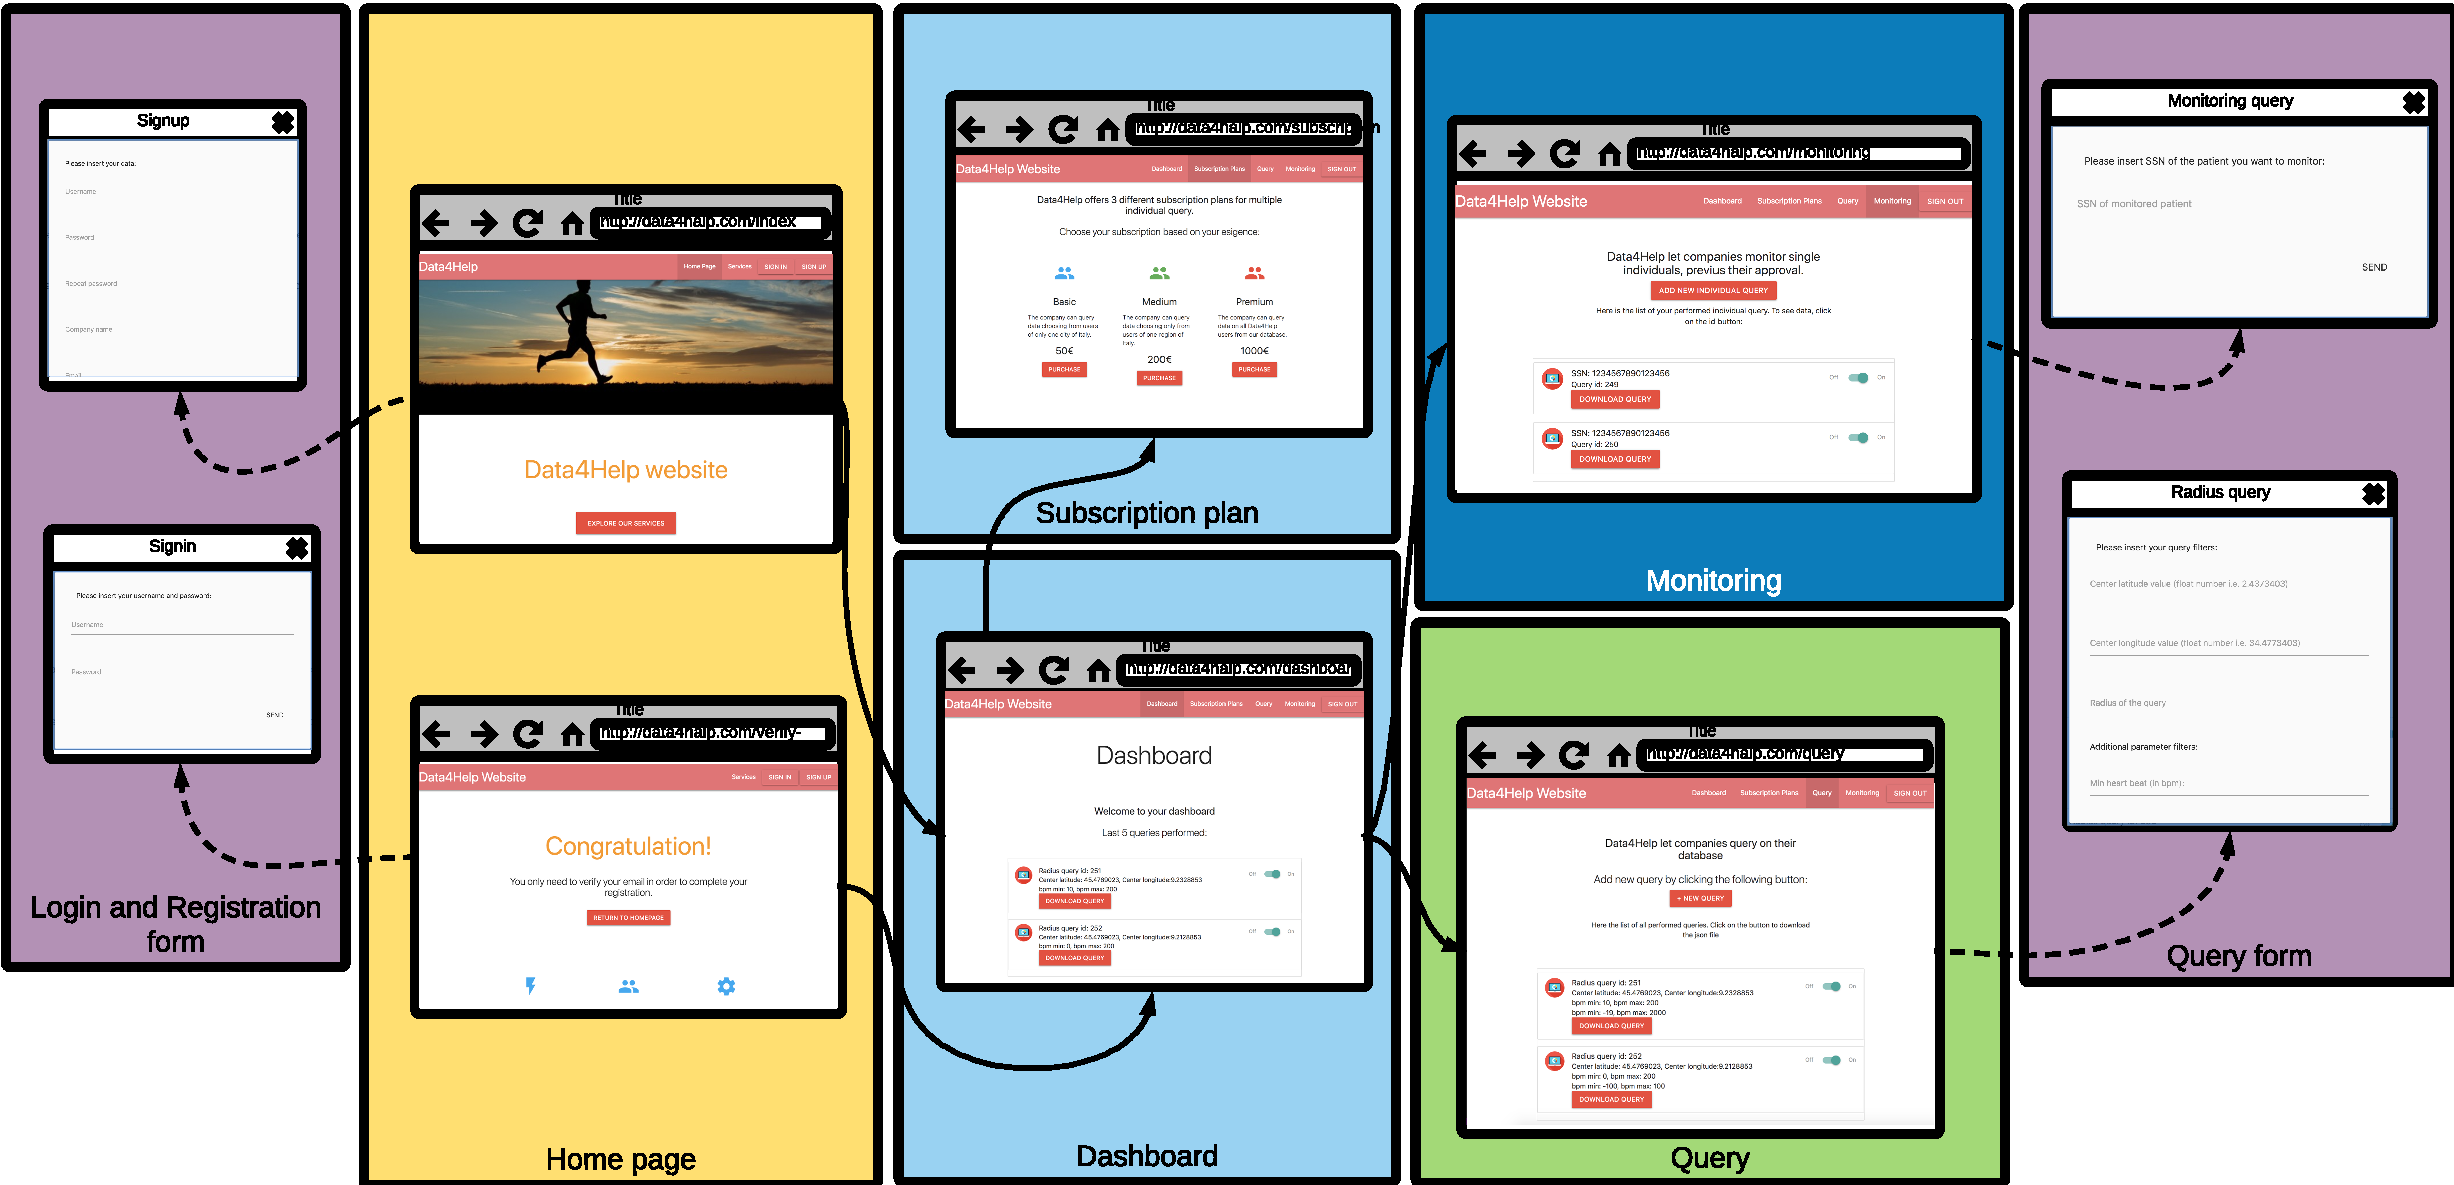
\includegraphics[width=\textwidth,height=\textheight,keepaspectratio]{assets/Website_Flow.pdf}
	\caption{Storyboard structure of the Website}
	\label{fig:StoryBoardWeb}
\end{figure}
The figure above shows the UI flow of the website.
It is dived in four parts:
\begin{itemize}
    \item \textbf{Home page}: allows the user to either login or sign up. If correctly signed up, shows a successful registration page;
    \item \textbf{Login and Registration form}: the forms that user compiles in order to register.
    \item \textbf{Dashboard}: the page where the user is redirected after correct login;
    \item \textbf{Query}: allows the company to perform a new query on a group of individual and to download the xml of the already performed queries.
    \item \textbf{Monitoring}: allows the company to perform a new query on individuals and to download the XML content of the already performed queries.
    \item \textbf{Query form}: the forms that user compiles in order to perform queries.

\end{itemize}



\subsection{Backend project structure}
This section aims at explaining the structure of the backend inside the \texttt{backend} directory.
Note that this section only briefly describes the directories and the files in it, for more detailed explainations it is advisable to look at the comments in the source code.

The root directory contains the following files: 
\begin{itemize}
    \item \texttt{app.js} The entry point of the app. It defines how to handle different endpoints, how to catch errors and starts the server.
    \item \texttt{dbdump} Current dump of the database.
    \item \texttt{start.sh} Start script.
    \item \texttt{jest.config.js} The configuration file for \texttt{jest}, the testing framework.
    \item \texttt{package.json} Lists all the dependencies needed for the program to run and various other informations on the application.
    \item \texttt{package-lock.json} Contains the state of the dependency tree of the application.
    \item  \texttt{Procfile} Contains the command to be run by Heroku to start the application.
\end{itemize}
And the following directories: 
\begin{itemize}
    \item \texttt{managers}: Contains the managers of the application.
    \item \texttt{routes}: Contains the routes definition for the application.
    \item \texttt{\_\_tests\_\_}: Contains the tests for the application. 
    \item \texttt{utils}: Contains some utilites function used during testing and debugging
    \item \texttt{stub\_endpoint}: Contains the stub of endpoint responses used during the initial phase of building the application.
    All the responses contain a success response and various error responses.
\end{itemize}

\subsubsection{managers}
The managers folder contains a single file: 
\begin{itemize}
    \item \texttt{config.js}: Allows to configure some parameters of the app, such as the minimum number of users for which allow a radius query, the database to connect to and the maximum amount of client allowed.
\end{itemize}

And the following folders with their respective files \\
\noindent \textbf{authentication}
\begin{itemize}
    \item \texttt{AuthenticationManager.js}: Handles login and registration of actors.
    \item \texttt{requiredParams.json}: Required parameters for login and registration of each actor.
\end{itemize}

\noindent \textbf{individual}
\begin{itemize}
    \item \texttt{IndividualsManager.js}: Handles post and retreival of individuals' data.
    \item \texttt{requiredParams.json}: Required parameters for the data posted.
\end{itemize}

\noindent \textbf{query}
\begin{itemize}
    \item \texttt{QueriesManager.js}: Handles post, retreival and performing of the companies' queries.
    \item \texttt{requiredParams.json}: Required parameters for the queries.
    \item \texttt{templateQueries.json}: Template queries for insertion in the database 
\end{itemize}

\noindent \textbf{runs}
\begin{itemize}
    \item \texttt{RunManager.js}: Handles creation, retrieval of a run, joining a run and monitoring participants in a run.
    \item \texttt{runStatus}: Exports the constans for the status of a run.
\end{itemize}

\noindent \textbf{subs}
\begin{itemize}
    \item \texttt{SubscriptionManager.js}: Handles the subscription. Not implemented.
\end{itemize}

\noindent \textbf{token}
\begin{itemize}
    \item \texttt{TokenManager.js}: Handles operations concerning the token, such as the retreival of the actor or the check of the presence of the user in a database.
\end{itemize}

\subsubsection{routes}
The routes folder contains a single file: 
\begin{itemize}
    \item \texttt{router.js}: Joins all the defined endpoints end exports the as a single endpoint.
\end{itemize}

\noindent And the folder \texttt{endpoints}, which contains the following files: 
\begin{itemize}
    \item \texttt{auth.js}: Exports the endpoints for authentication. Handles login and registration of actors via the use of the functions declared in the \texttt{AuthenticationManager.js} file.
    \item \texttt{indiv.js}: Exports the endpoints for the individual. Handles post and retrival of individuals' data via the functions declared in the \texttt{IndividualsManagers.js} file.
    \item \texttt{queries.js}: Exports the endpoints for the queries. Handles post and retrival of company queries via the functions declared in the \texttt{QueriesManager.js} file.
    \item \texttt{runs.js}: Exports the endpoints for the runs management.  Handles post and retrival of run organizers run, subscription of individuals to a run, monitoring of runners in a run via the functions declared in the \texttt{RunsManager.js} file.
    \item \texttt{subs.js}: Exports the endpoints for subscription to query plans. Not implemented.

\end{itemize}

\subsubsection{\_\_tests\_\_}
The routes folder contains a single file: 
\begin{itemize}
    \item \texttt{config.js}: Internal configuration for the tests. Exports the token for company, run organizer, individual their mail and their password. Additionally it exports the URL on which perform the tests.
\end{itemize}

\noindent And the following directories with their respective files: \\
\noindent \textbf{auth}
\begin{itemize}
    \item \texttt{featureTest.jest.js}: Feature tests for the /auth endpoint
    \item \texttt{unitTest.jest.js}: Unit tests for the helper functions of \texttt{AuthenticationManager.js}
\end{itemize}
\noindent \textbf{indiv}
\begin{itemize}
    \item \texttt{featureTest.jest.js}: Feature tests for the /indiv endpoint
    \item \texttt{unitTest.jest.js}: Unit tests for the helper functions of \texttt{IndividualsManager.js}
\end{itemize}
\noindent \textbf{query}
\begin{itemize}
    \item \texttt{featureTest.jest.js}: Feature tests for the /queries endpoint
    \item \texttt{unitTest.jest.js}: Unit tests for the helper functions of \texttt{QueriesManager.js}
\end{itemize}
\noindent \textbf{runs}
\begin{itemize}
    \item \texttt{featureTest.jest.js}: Feature tests for the /runs endpoint
    \item \texttt{unitTest.jest.js}: Unit tests for the helper functions of \texttt{RunsManager.js}

\end{itemize}


\subsubsection{stub\_endpoint}
Contains the following folders: 

\noindent \textbf{auth}
\begin{itemize}
    \item \texttt{login.json}: Mock response on enpoint \texttt{/auth/login}.
    \item \texttt{register\_company.json}: Mock response on enpoint \texttt{/auth/register\_company}.
    \item \texttt{register\_run\_organizer.json}: Mock response on enpoint \texttt{/auth/register\_run\_organizer}.
    \item \texttt{register\_user.json}: Mock response on enpoint \texttt{/auth/register\_user}.
    \item \texttt{verify.json}: Mock response on enpoint \texttt{/auth/verify}.

\end{itemize}

\noindent \textbf{indiv}
\begin{itemize}
    \item \texttt{data\_POST.json}: Mock response for the POST request on endpoint \texttt{/indiv/data}.
    \item \texttt{data\_GET.json}: Mock response for the GET request on endpoint \texttt{/indiv/data}.
\end{itemize}

\noindent \textbf{query}
\begin{itemize}
    \item \texttt{query\_POST.json}: Mock response for the POST request on endpoint \texttt{/queries/query}.
    \item \texttt{query\_GET.json}: Mock response for the GET request on endpoint \texttt{/queries/query}.
\end{itemize}


\noindent \textbf{runs}
\begin{itemize}
    \item \texttt{join.json}: Mock response for the POST request on endpoint \texttt{/runs/join}.
    \item \texttt{positions.json}: Mock response for the GET request on endpoint \texttt{/runs/positions}.
     \item \texttt{root.json}: Mock response for the POST request on endpoint \texttt{/runs/}.
    \item \texttt{run.json}: Mock response for the GET request on endpoint \texttt{/runs/run}.
\end{itemize}

\noindent \textbf{subs}
\begin{itemize}
     \item \texttt{plan\_GET.json}: Mock response for the POST request on endpoint \texttt{/subs/plan}. Still active.
    \item \texttt{plan\_POST.json}: Mock response for the POST request on endpoint \texttt{/runs/positions}.
\end{itemize}

\subsubsection{utils}
Contains a single file: 
\begin{itemize}
    \item \texttt{testUtils.js} Utilities function used during testing.
\end{itemize}


